\section{SD卡的驱动框架}
6.2.1 SD/MMC卡介绍

1.1.什么是MMC卡

MMC:MMC就是MultiMediaCard的缩写,即多媒体卡。它是一种非易失性存储器件,体积小巧(24mm*32mm*1.4mm),容量大,耗电量低,传输速度快,广泛应用于消费类电子产品中。

1.2.什么是SD卡

SD:SD卡为Secure Digital Memory Card, 即安全数码卡。它在MMC的基础上发展而来,增加了两个主要特色:SD卡强调数据的安全安全,可以设定所储存的使用权限,防止数据被他人复制;另外一个特色就是传输速度比2.11版的MMC卡快。在数据传输和物理规范上,SD卡(24mm*32mm*2.1mm,比MMC卡更厚一点),向前兼容了MMC卡.所有支持SD卡的设备也支持MMC卡。SD卡和2.11版的MMC卡完全兼容。
\begin{figure}[H]
    \centering
    \scalebox{0.5}{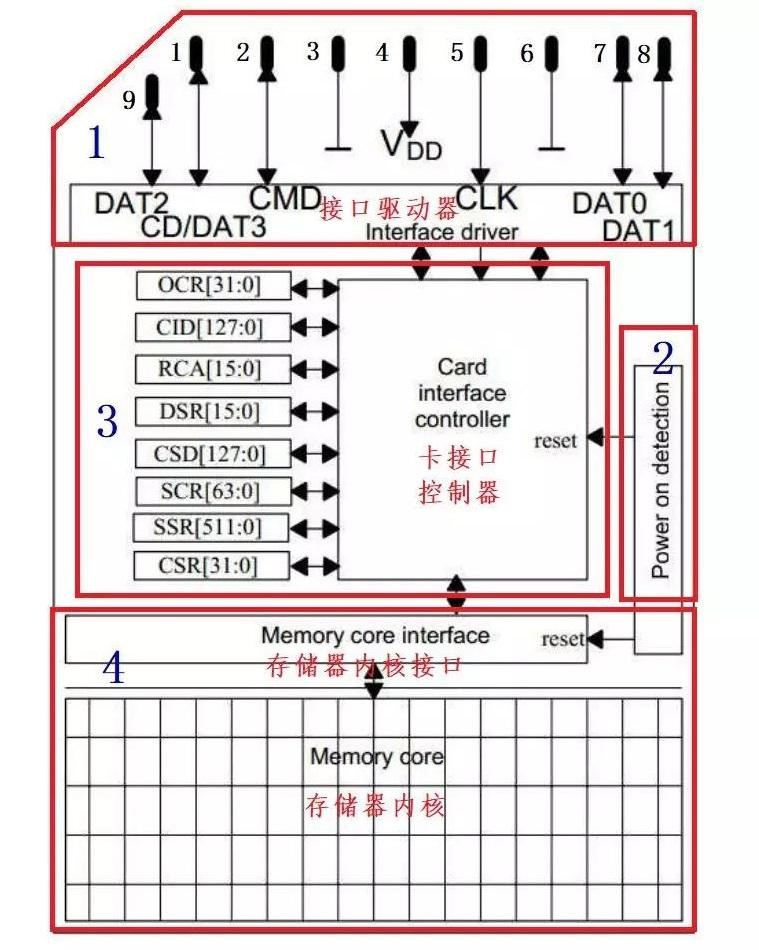
\includegraphics{figures/06-02-SD.jpg}}
    \caption{6-2-1. SD卡内部结构}
\end{figure}

SD卡内部结构如上图所示

1.3.什么是SDIO

SDIO:SDIO是在SD标准上定义了一种外设接口,它和SD卡规范间的一个重要区别是增加了低速标准。在SDIO卡只需要SPI和1位SD传输模式。低速卡的目标应用是以最小的硬件开销支持低速IO能力。

1.4.什么是MCI

MCI:MCI是Multimedia Card Interface的简称,即多媒体卡接口。上述的MMC,SD,SDI卡定义的接口都属于MCI接口。MCI这个术语在驱动程序中经常使用,很多文件,函数名字都包括”mci”.

1.5.MMC/SD/SDIO卡的区别


\begin{tabular}{|c|c|c|c|}
    
    \hline
    卡属性&引脚个数&宽度&长度&厚度&SPI传输模式&1位传输模式&时钟频率&最高传输率&最高SPI传输率\\
    \hline
    MMC卡&7&24mm&32mm&1.4mm&可选&是&否&0-20MHz&20Mbit/s&20Mbit/s \\
    \hline
    SD卡&9&24mm&32mm&2.1mm&支持&是&可选&0-25MHz&100Mbit/s&25Mbit/s \\
    \hline
    SD卡&9&24mm&32mm+&2.1mm&支持&是&可选&0-25MHz&100Mbit/s&25Mbit/s \\
    \hline
  \end{tabular}

SD卡内部有7个寄存器,如下表1所示.其中OCR,CID,CSD和SCR寄存器保存卡的配置信息;RCA寄存器保存着通信过程中卡当前暂时分配的地址(只适合SD模式);卡状态(Card Status)和SD状态(SD Status)寄存器保存着卡的状态(例如,是否写成功,通信的CRC校验是否正确等),这两个寄存器的内容与通信模式(SD模式或SPI模式)相关.MMC卡没有SCR和SD Status寄存器.

\begin{tabular}{|c|c|c|}    

    \hline
    名字 & CID & RCA & DSR & SCR & OCR &SSR &CSR \\
    \hline
    宽度 & 128 & 16 & 16 & 128 & 64 & 32 & 512 & 32 \\
    \hline
    卡识别号,每张卡都有的唯一识别号 & 发布卡的地址,卡的局部系统地址,在初始化过程中,由主机和卡动态支持 & 驱动级寄存器,配置卡的驱动输出 &
    卡的协议数据,关于卡的操作状态数据 & 卡配置寄存器,关于卡特性容量的信息 & 操作状态寄存器&
    SD状态,有关卡拥有的特性信息 & 卡状态,有关卡状态的信息 \\
    \hline
\end{tabular}

OCR寄存器保存着SD/MMC卡的供电电允许范围.如下表2所示:如果OCR寄存器的某位为1,表示卡支持该位对应的电压。最后一位表示卡上电后的状态(是否处于”忙状态”),如果该位为0,表示忙,如果为1,表示处于空闲状态(MMC/SD协议P60)。


\begin{tabular}{|c|c|}
    \hline
    OCR~bit~position&0-3&4&5&6&7&8&9&10&11&12&13&14&15&16&17&18&19&20&21&22&23&24-30&31\\
    \hline
    VDD~votage~window & Reserved & 1.6-1.7 & 1.7-1.8 & 1.8-1.9 & 1.9-2.0 & 2.0-2.1 & 2.1-2.2 & 2.2-2.3 &
    2.3-2.4 & 2.4-2.5 & 2.5-2.6 & 2.6-2.7 & 2.7-2.8 & 2.8-2.9 & 2.9-3.0 & 3.0-3.1 & 3.1-3.2 &
    3.2-3.3 & 3.3-3.4 & 3.4-3.5 & 3.5-3.6 & Reserved & Card~power~up~status~bit~(busy)1 \\
    \hline
\end{tabular}

CID为一个16个字节的寄存器,该寄存器包含一个独特的卡标识号。如下表所示:


\begin{tabular}{|c|c|c|c|}
    \hline
    Name&Manufacturer~ID&OEM/Application~ID&Product~name&Product~Revision&Product~Serial~Number&Reserved&Manufacturing~Date&CRC7~Checksum&not~used,~always~"T"\\
    \hline
Field&
MID&
OID&
PNM&
PRV&
PSN&
...&
MDT&
CRC&
-\\
    \hline
    Width&
8&
18&
40&
8&
32&
4&
12&
7&
1\\
    \hline
CID-slice&
[127:120]&
[119:104]&
[103:64]&
[83:56]&
[55:24]&
[23:20]&
[19:8]&
[7:1]&
[0:0]\\
    \hline
\end{tabular}

SD/SDIO有以下几种传输模式:
(1)SPI mode,独立序列输入和独立序列输出,使⽤CS、DI、SCLK与DO(SD卡的片选、数据输入、
时钟与数据输出)四根信号线进行数据传输。

(2)1-bit mode,独立指令和数据通道,只支持1位宽的数据传输。

(3)4-bit mode,使用额外的针脚以及某些重新设置的针脚。支持四位宽的并行传输。

6.2.2 k210联动SD卡

K210 裸机使用SD卡,下图是SD卡对应接口
\begin{figure}[H]
    \centering
    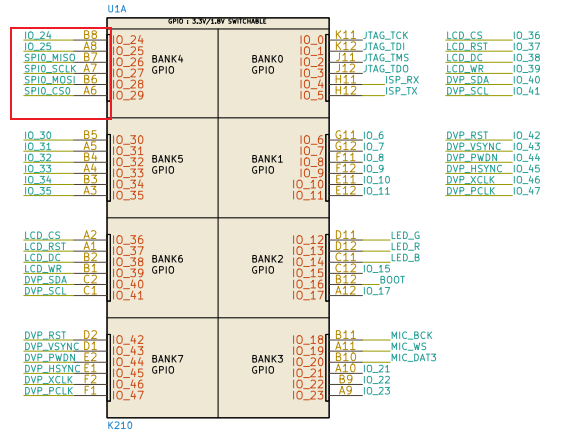
\includegraphics{figures/06-02-接口标.png}
    \caption{6-2-2. SD卡与K210接口}
\end{figure}

为了协同软硬接口,我们需要在代码中定义相关常量,使软硬接口保持一致,这即为遵守SD卡协议。
\begin{lstlisting}[language={Rust}, label={code:inode},
	caption={SD卡协议}]
    const MMIO =[
        (0x0C00_0000, 0x3000), /* PLIC */
        (0x0C20_0000, 0x1000), /* PLIC */
        (0x3800_0000, 0x1000), /* UARTHS */
        (0x3800_1000, 0x1000), /* GPIOHS */
        (0x5020_0000, 0x1000), /* GPIO */
        (0x5024_0000, 0x1000), /* SPI_SLAVE */
        (0x502B_0000, 0x1000), /* FPIOA */
        (0x502D_0000, 0x1000), /* TIMER0 */
        (0x502E_0000, 0x1000), /* TIMER1 */
        (0x502F_0000, 0x1000), /* TIMER2 */
        (0x5044_0000, 0x1000), /* SYSCTL */
        (0x5200_0000, 0x1000), /* SPI0 */
        (0x5300_0000, 0x1000), /* SPI1 */
        (0x5400_0000, 0x1000), /* SPI2 */
        ];
\end{lstlisting}


应用程序通过文件系统接口如open()、read()、write()、close()等访问文件系统,根据文件系统inode节点,接着找到文件在SD卡驱动上的块号。文件系统通过块设备驱动层与SD卡协议层对接,块设备驱动层定义了抽象块设备的接口,主要包括对块设备的读写接口。SD卡协议层主要负责按照SD卡标准规范向SD卡发送指令或者接收响应数据;硬件接口层则负责按照硬件板卡的引脚定义操作GPIO或SPI引脚实现与SD卡的数据交互。

6.2.3 SD卡的命令
 
SD卡命令共分为12类,分别为class0到Class11.
 
3.2.1. Class0 :(卡的识别、初始化等基本命令集)
CMD0:复位SD 卡。

CMD1:读OCR寄存器。

CMD9:读CSD寄存器。

CMD10:读CID寄存器。

CMD12:停止读多块时的数据传输。

CMD13:读 Card_Status 寄存器。

3.2.2.Class2 (读卡命令集):

CMD16:设置块的长度。

CMD17:读单块。

CMD18:读多块,直至主机发送CMD12为止 。
 
3.2.3.Class4(写卡命令集) :

CMD24:写单块。

CMD25:写多块。

CMD27:写CSD寄存器 。

3.2.4.Class5 (擦除卡命令集):

CMD32:设置擦除块的起始地址。

CMD33:设置擦除块的终止地址。

CMD38: 擦除所选择的块。


3.2.5.Class6(写保护命令集):

CMD28:设置写保护块的地址。

CMD29:擦除写保护块的地址。

CMD30: Ask the card for the status of the write protection bits

 class7:卡的锁定,解锁功能命令集。

 class8:申请特定命令集 。

 class10 -11 :保留。

(注:完整细节请自行参考SD卡协议官方文档)

6.2.4 SD卡工作流程

SD卡工作流程大致可以分为3个大的步骤:初始化sd卡、写sd卡、读sd卡。在SPI模式下,SD卡工作模式分为卡识别模式和数据传输模式。如下图为卡在识别模式下的命令流程。

\begin{figure}[H]
    \centering
    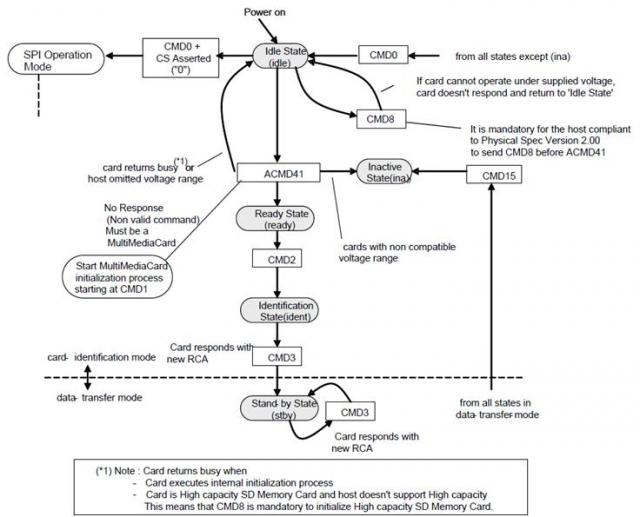
\includegraphics{figures/06-02-命令流程.png}
    \caption{6-2-3. 卡识别模式命令流程}
\end{figure}

在复位后,查找总线上的新卡的时候,主机会处于“卡识别模式”。卡在复位后会处于识别模式。不同的SD卡可能支持不同版本的协议或者不同的⼯作电压。因此,作为主机,在与SD卡进行交互之初,主机需要获取卡的工作电压范围和卡的类型。在卡识别期间,时钟频率应该保持在100~400kHZ之间。

1_在主机和SD卡进行任何通信之前,主机不知道SD卡支持的工作电压范围,卡也不知道是否支持主机当前提供的电压。因此主机首先使用默认的电压发送一条reset指令(CMD0)。

2_为了验证SD卡的接口操作状态,主机发送SEND_IF_COND(CMD8),用于取得SD卡支持工作的电压范围数据。SD卡通过检测CMD8的参数部分来检查主机使用的工作电压,主机通过分析回传的CMD8参数部分来校验SD卡是否可以在所给电压下工作,如果SD卡可以在指定电压下工作,则它回送CMD8的命令响应字 。如果不支持所给电压,则SD卡不会给出任何响应信息,并继续处于IDLE状态。

3_在发送ACMD41命令初始化高容量的SD卡前,需要强制发送CMD8命令。强制低电压主机在发送CMD8前发送ACMD41,万一双重电压SD卡没有收到CMD8命令且工作在高电压状态,在这种情况下,低电压主机不能不发送CMD8命令给卡,则收到ACMD41后进入无活动状态。

4_SD_SEND_OP_COND(ACMD)命令是为SD卡主机识别卡或者电压不匹配时拒绝卡的机制设计的。主机发送命令操作数代表要求的电压窗口大小。如果SD卡在所给的范围内不能实现数据传输,将放弃下一步的总线操作而进入无活动。操作状态寄存器也将被定义。

5_在主机发出复位命令(CMD0)后,主机将先发送CMD8再发送ACMD41命令重新初始化SD卡。

当总线被激合后,主机就开始卡的初始化和识别3处理。初始化处理设置它的操作状态和是设置OCR中的HCS比特命令SD_SEND_OP_COND(ACMD41)开始。HCS比特位被设置为1表示主机支持高容量SD卡。HCS被设置为0表示主机不支持高容量SD卡。卡的初始化和识别流程见下图。
\begin{figure}[H]
    \centering
    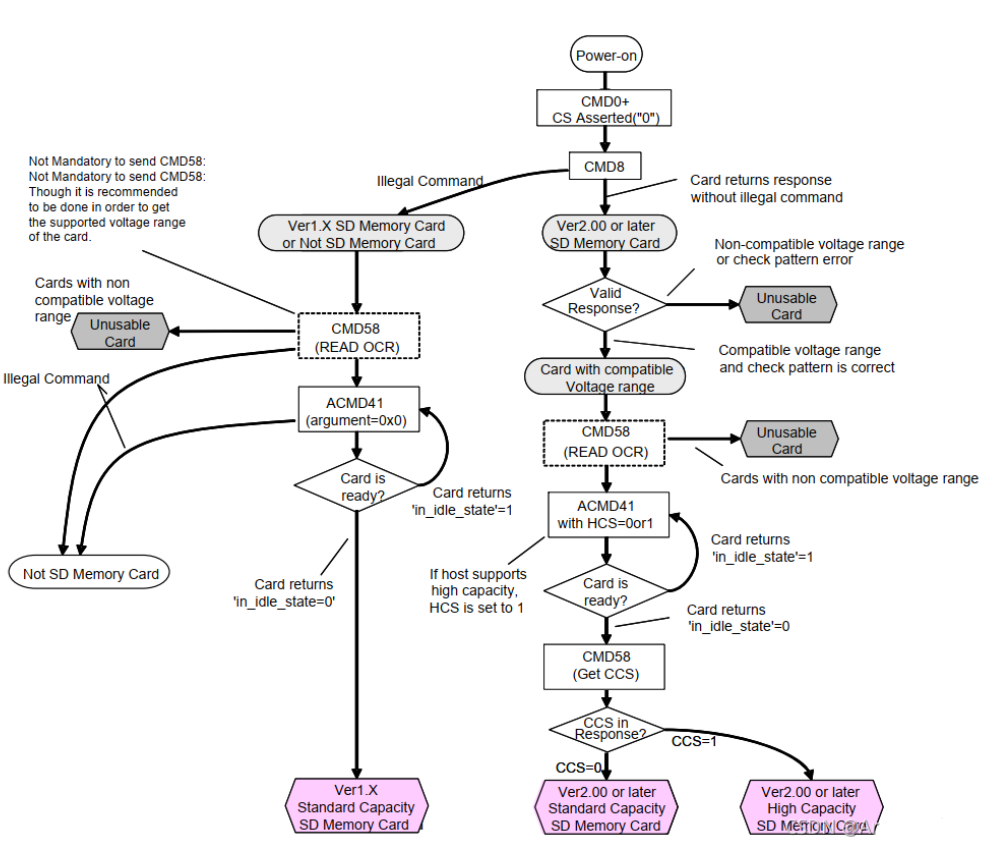
\includegraphics{figures/06-02-初始化.png}
    \caption{6-2-4. 卡初始化和识别流程}
\end{figure}
(注:这里不推荐使用NPUCore或rCore作为代码范式来讲解,应直接看SD卡协议文档)

卡在识别模式结束后,主机时钟fpp(数据传输时钟频率)将保存为fod(卡识别模式下的时钟),由于有些卡对操作时钟有限制。主机必须发送SEND_CSD(CMD9)来获得卡规格数据积存器内容,如块大小,卡容量。广播命令SET_DSR(CMD4)配置所有识别卡的驱动阶段。它对DSR积存器进行编程以适应应用总线布局,总线上的卡数目和数据传输频率。SD卡数据传输模式的流程图如下图。
\begin{figure}[H]
    \centering
    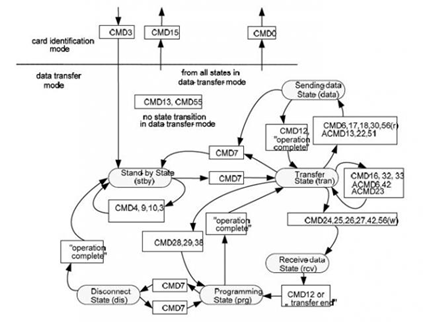
\includegraphics{figures/06-02-数据传输.png}
    \caption{6-2-5. 卡数据传输模式流程}
\end{figure}

1CMD7命令用来选择某个SD卡,使其进入Transfer状态,在指定时间段内,只有一个卡能处于Transfer状态。当某个先前被选中的处于Transfer状态的SD卡接收到CMD7之后,会释放与控制器的连接,并进入Stand-by态。当CMD7使用保留地址0x0000时,所有的SD卡都会进入Stand-by状态 。


2所有的数据读命令都可以被停止命令(CMD12)在任意时刻终止。数据传输会终止,SD卡返回Transfer状态。读命令有:块读操作(CMD17)、多块读操作(CMD18)、发送写保护(CMD30)、发送scr(ACMD51)以及读模式下的普通命令(CMD56)。

3所有的数据写命令都可以被停止命令(CMD12)在任意时刻终止。写命令也会在取消选择命令(CMD7)之前停止。写命令有:块写操作(CMD24,CMD25)、编程命令(CMD27)、锁定/解锁命令(CMD42)以及写模式下的普通命令(CMD56)。

4数据传输一旦完成,SD卡会退出数据写状态,进入Programming状态(传输成功)或者Transfer状态(传输失败)。
